\documentclass[aps,prl,preprint]{revtex4-1}
\usepackage{amsmath,amsfonts,amssymb}
\usepackage{graphicx}
\usepackage{comment}
\usepackage{subcaption}
\usepackage{hyperref}
\usepackage{braket}

\newcommand{\midrule}{\hline}
\newcommand{\bottomrule}{\hline\hline}
\newcommand{\bs}{\boldsymbol}

\usepackage{xcolor,framed}
\definecolor{shadecolor}{gray}{0.95}
% \verb|ax.plot(x,y)| for inline code
% \begin{shaded}\begin{verbatim} for block code
% \begin{subfigure}{0.48\textwidth} for subfigure

\begin{document}
\section{Simple Harmonic Oscillator in 1D}

\subsection{Exercise 1: Exact Density Matrix}
The simple harmonic oscillator (SHO) in 1D is modeled by the Hamiltonian
\begin{align}
\hat{\mathcal{H}} = -\frac{\hbar^2}{2m}\frac{\partial^2}{\partial x^2} + \frac{1}{2}m\omega^2x^2.
\end{align}
Its density matrix(DM) is given by the Bloch equation
\begin{align}
-\frac{\partial \rho(x,x';\beta)}{\partial \beta} = \hat{\mathcal{H}}\rho(x,x';\beta),
\end{align}
with the initial condition $\rho(x,x';0)=\delta(x-x')$. The solution 
\begin{align}
\rho(x,x';\beta) = \sqrt{\frac{m\omega}{2\hbar\sinh(\hbar\beta\omega)}/\pi}
\exp\left\{ -\frac{m\omega}{2\hbar\sinh(\hbar\beta\omega)} \left[ (x^2+x'^2)\cosh(\hbar\beta\omega)-2xx' \right] \right\}.
\end{align}
Use atomic units ($\hbar=1$) and define $A\equiv\frac{m\omega}{2\sinh(\beta\omega)}$, then
\begin{align}
\rho(x,x';\beta) = \sqrt{A/\pi}
\exp\left\{ -A \left[ (x^2+x'^2)\cosh(\beta\omega)-2xx' \right] \right\}. \label{eq:exact_dm}
\end{align}
The SHO can be completely characterized by its mean squared fluctuation
\begin{align}
\boxed{\braket{x^2} =\frac{\int dx x^2 \rho(x,x;\beta)}{\int dx \rho(x,x;\beta)} = \frac{\hbar}{2m\omega}\coth(\frac{\hbar\beta\omega}{2})}. \label{eq:exact_x2}
\end{align}
The potential energy $\braket{V}=\frac{1}{2}m\omega^2\braket{x^2}$, and the total energy is given by the Virial theorem. Define action $S\equiv-\ln\rho$ and ignore the normalization of $\rho$, then the \emph{exact link action}
\begin{align} 
S_e(x,x';\beta) = A\left[(x^2+x'^2)\cosh(\beta\omega)+2xx'\right].\label{eq:exact_link_action}
\end{align}
Notice, if temperature is high $\beta=\tau\approx0$, then eq.~(\ref{eq:exact_link_action}) reduces to the \emph{primitive link action}
\begin{align} 
S_p(x,x';\tau) = \tau \left[\frac{1}{2} m\left(\frac{x-x'}{\tau}\right)^2\right] +\frac{\tau}{2}\left[\frac{1}{2}m\omega^2(x^2+x'^2) \right].
\end{align}
An algorithm that performs eq.~(\ref{eq:exact_x2}) with Monte Carlo sampling is equivalent to path integral Monte Carlo (PIMC) with one time slice. MC sampling of the diagonal of the density matrix $\rho(x,x;\beta)$ can be performed with Metropolis algorithm using acceptance probability
\begin{align}
\mathcal{A} = \min\left(1,\exp -\Delta S_e \right).
\end{align}

\subsection{Exercise 2: Path Integral Construction of the Density Matrix}

The exact density matrix at low temperature $\beta$ can be constructed exactly as a convolution of $M$ high temperature $\tau=\beta/M$ density matrices
\begin{align}
\rho(x,x';\beta) = \int dx_1\dots dx_{M-1}~ \rho(x,x_1;\tau)\rho(x_1,x_2;\tau)\dots\rho(x_{M-1},x';\tau). \label{eq:pidm}
\end{align}

\begin{figure}[h]
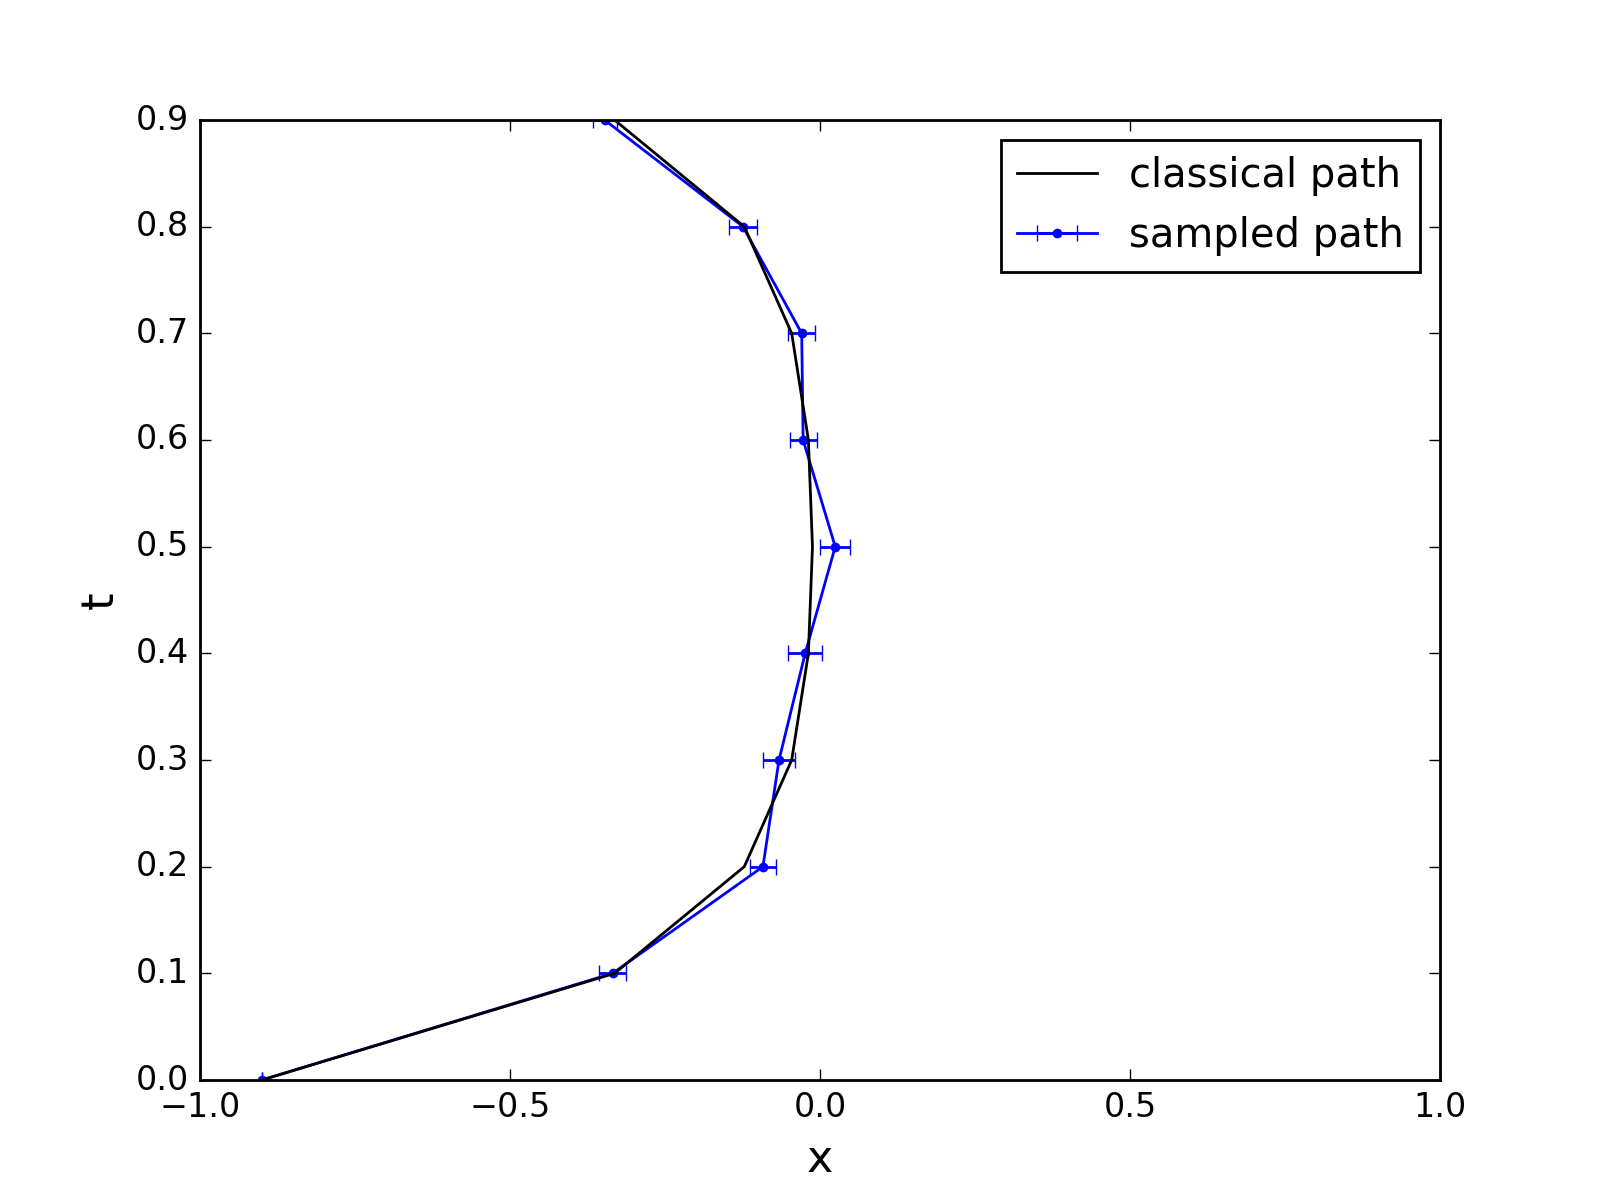
\includegraphics[scale=0.3]{figures/classical_path}
\caption{Path going from $x=x'=-0.9$\label{fig:classical_path}}
\end{figure}

The collection of \emph{time slices} $x_j$ can be thought of a trajectory through imaginary time $x_j\equiv x(t=j\tau)$. Then eq.~(\ref{eq:pidm}) is a functional integral over the space of imaginary-time \emph{paths} $x(t)$ as shown in Fig.~\ref{fig:classical_path}. Each path has an associated \emph{action} that determines its likelihood
\begin{align}
S[\left\{x_j\right\}] = \sum_{j=0}^{M-1} S_e(x_{j},x_{j+1};\tau),\text{ where } x_0\equiv x, x_M\equiv x'.
\end{align}
When $\tau\rightarrow0$, $x_{j}+1\approx x_j$, thus eq.~(\ref{eq:exact_link_action}) simplifies to
\begin{align}
S_e(x,\dot{x},t=j\tau) = \tau \left[ \frac{1}{2}m\dot{x}(t)^2 + \frac{1}{2}m\omega^2x(t)^2 \right],
\end{align}
which is reminiscent of the Lagrangian density. The paths from $x$ to $x'$ can be sampled with Metropolis. The classical path, which minimizes the action, will be sampled most often.

\subsection{Exercise 3: Path Integral Monte Carlo with Exact Link Action}



\end{document}
